\documentclass{standalone}
\usepackage{tikz}
\usetikzlibrary{shapes, positioning, calc}

\begin{document}

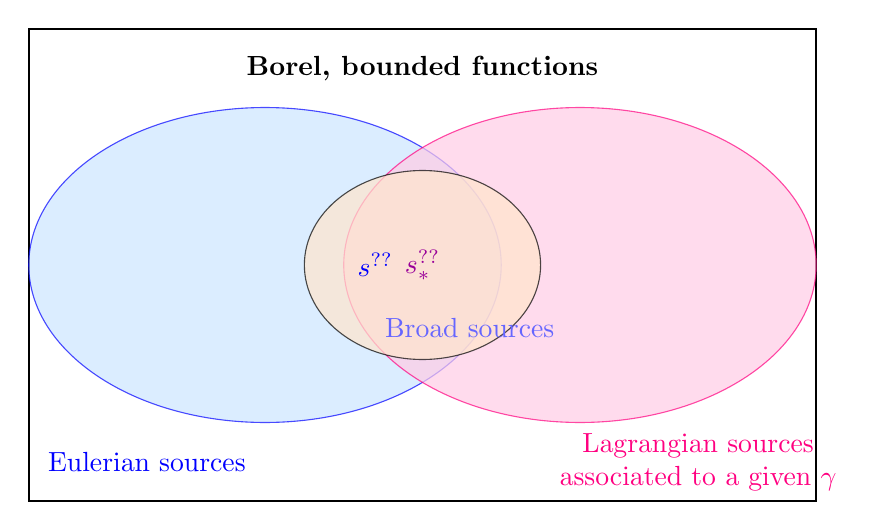
\begin{tikzpicture}
  % Define colors
  \definecolor{lightblue}{RGB}{204,229,255}
  \definecolor{lightpink}{RGB}{255,204,229}
  \definecolor{lightorange}{RGB}{255,229,204}
  \definecolor{blue}{RGB}{0,0,255}
  \definecolor{magenta}{RGB}{255,0,128}
  \definecolor{purple}{RGB}{153,0,153} % For intersection shade
  
  % Draw the outer rectangle
  \draw[thick] (-5,-3) rectangle (5,3);
  
  % Title
  \node[font=\bfseries] at (0,2.5) {Borel, bounded functions};
  
  % Draw the left ellipse (Eulerian sources)
  \filldraw[draw=blue, fill=lightblue, opacity=0.7] (-2,0) ellipse (3cm and 2cm);
  
  % Draw the right ellipse (Lagrangian sources)
  \filldraw[draw=magenta, fill=lightpink, opacity=0.7] (2,0) ellipse (3cm and 2cm);
  
  % Add the intersection fill (light orange with slight blend)
  \filldraw[fill=lightorange, opacity=0.7] (0,0) ellipse (1.5cm and 1.2cm);
  
  % Add labels
  \node[blue] at (-3.5,-2.5) {Eulerian sources};
  \node[magenta, align=center] at (3.5,-2.5) {Lagrangian sources\\associated to a given $\gamma$};
  
  % Add the text in the intersection
  \node[blue] at (-0.6,0) {$s^{??}$};
  \node[purple] at (0,0) {$s_*^{??}$};
  \node[blue!60] at (0.6,-0.8) {Broad sources};
\end{tikzpicture}

\end{document}